\documentclass[tikz,border=10pt]{standalone}

\begin{document}
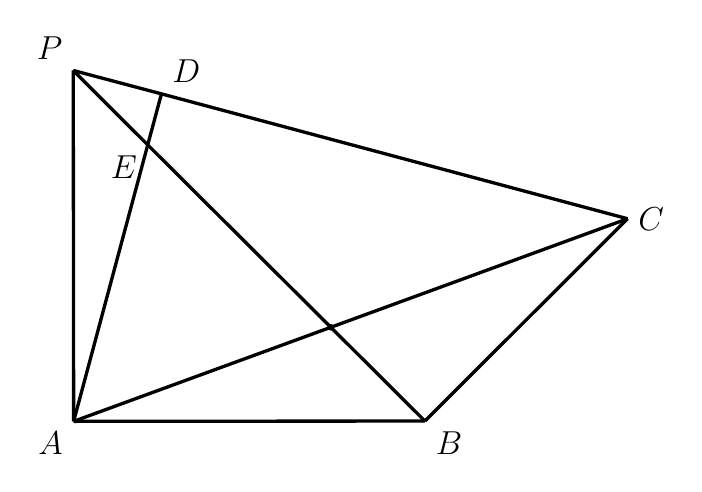
\begin{tikzpicture}[line join=round, line width=1.2pt]
\coordinate (A) at (-3.526,-2.377);
\coordinate (B) at (0.935,-2.373);
\coordinate (C) at (3.509,0.196);
\coordinate (D) at (-2.411,1.782);
\coordinate (E) at (-2.585,1.134);
\coordinate (P) at (-3.531,2.079);

  
  \draw (P) -- (A);
  \draw (A) -- (B);
  \draw (P) -- (E) -- (B);
  \draw (P) -- (D) -- (C);
  \draw (A) -- (C);
  \draw (B) -- (C);
  \draw (A) -- (E) -- (D);

  
  \fill (-0.261,-1.182) circle (1.200pt);

  
  \node[above left, font=\fontsize{12.5}{15}\selectfont] at (P) {$P$};
  \node[below left, font=\fontsize{12.5}{15}\selectfont] at (A) {$A$};
  \node[below right, font=\fontsize{12.5}{15}\selectfont] at (B) {$B$};
  \node[right, font=\fontsize{12.5}{15}\selectfont] at (C) {$C$};
  \node[above right, font=\fontsize{12.5}{15}\selectfont] at (D) {$D$};
  \node[below left, font=\fontsize{12.5}{15}\selectfont] at (E) {$E$};
\end{tikzpicture}
\end{document}